\subsection{Transparency}\label{subsec:introduction--transparency}

\enlargethispage{\baselineskip}
\renewcommand{\bottomfraction}{0.85}
\renewcommand{\topfraction}{0.85}
\renewcommand{\textfraction}{0.1}

A distributed system should \hl{hide unnecessary aspects of distribution so that users and programmers can interact with it more simply.} Transparency is largely about achieving the \textbf{illusion} that the system is a single, coherent entity. The user should not have to reason about every server, replica, physical location, migration, or failure unless that information is actually important.

\hfill

\begin{figure}[!htp]
    \centering
    \tikzsetnextfilename{transparency-membrane}
    \begin{tikzpicture}[
            font=\footnotesize,
            execute at begin node={\hyphenpenalty=10000 \exhyphenpenalty=10000 },
            userbox/.style={
                rounded corners=6pt, draw=blue!75!black, fill=blue!6, thick,
                text width=8.8cm, align=center, inner sep=6pt
            },
            layerbox/.style={
                rounded corners=6pt, draw=teal!80!black, fill=teal!8, thick, dashed,
                text width=10.9cm, align=center, inner sep=6pt
            },
            nodebox/.style={
                rounded corners=4pt, draw=gray!70!black, fill=white, thick,
                text width=3.1cm, minimum height=1.9cm, align=center, inner sep=4pt
            },
            failbox/.style={nodebox, draw=red!75!black, fill=red!6, dashed},
            arr/.style={->, very thick, blue!80!black, >=Stealth},
            syncwire/.style={<->, thick, purple!75!black, dashed, >=Stealth},
            failwire/.style={->, very thick, red!75!black, >=Stealth}
        ]

        % --- Top: logical view of the client ---
        \node[userbox] (client) at (0, 8.0) {
            \textbf{\textcolor{blue!80!black}{\faIcon{laptop-code}} Logical illusion: one coherent system}\\[3pt]
            \texttt{data = resource.get("customer\_42")}\\[2pt]
            {\color{gray!80!black}The client sees one abstraction, not the topology}
        };

        % --- Middle: the transparency membrane ---
        \node[layerbox] (membrane) at (0, 5.3) {
            \textbf{\textcolor{teal!90!black}{\faIcon{layer-group}} Transparency membrane}\\[1pt]
            {\scriptsize (middleware / distributed OS)}\\[3pt]
            hides \emph{where} (location) $\cdot$ hides \emph{format} (access)\\
            picks a copy (replication) $\cdot$ masks crashes (failure)
        };

        \draw[arr] (client.south) -- (membrane.north)
        node[midway, right=6pt, font=\footnotesize\bfseries, text=blue!80!black] {logical method call};

        % --- Physical reality ---
        \draw[rounded corners=7pt, fill=gray!3, draw=gray!35, thick] (-5.85, -5.0) rectangle (5.85, 3.55);

        \node[anchor=south west, align=left, text=gray!75!black] at (-5.65, -4.9) {
            \faIcon{server} \textbf{Physical hosts}\\
            {\scriptsize heterogeneous}
        };
        \node[anchor=south east, align=right, text=red!75!black] at (5.65, -4.9) {
            \faIcon{exclamation-triangle} \textbf{Fault-prone}\\
            {\scriptsize crashes \& partitions}
        };

        % --- Top row: replicas ---
        \node[nodebox] (n2) at (-3.0, 0.5) {
            \textbf{Node $C_2$}\\[1pt]
            {\scriptsize\color{gray!70!black}\faIcon{microchip} ARM / Cloud}\\[2pt]
            {\color{purple!80!black}Replica $R_1$}\\[1pt]
            {\scriptsize Milan}
        };
        \node[nodebox] (n3) at (3.0, 0.5) {
            \textbf{Node $C_3$}\\[1pt]
            {\scriptsize\color{gray!70!black}\faIcon{microchip} x86 / Cloud}\\[2pt]
            {\color{purple!80!black}Replica $R_2$}\\[1pt]
            {\scriptsize Frankfurt}
        };

        % --- Bottom row: old home and crashed node ---
        \node[nodebox] (n1) at (-3.0, -2.8) {
            \textbf{Node $C_1$}\\[1pt]
            {\scriptsize\color{gray!70!black}\faIcon{microchip} x86 / Linux}\\[2pt]
            {\color{teal!80!black}$R$ (old home)}
        };
        \node[failbox] (n4) at (3.0, -2.8) {
            \textbf{Node $C_4$}\\[1pt]
            {\scriptsize\color{red!80!black}\faIcon{times-circle} crashed}\\[2pt]
            {\color{red!80!black}Replica $R_3$}\\[1pt]
            {\scriptsize unreachable}
        };

        % --- Arrows ---
        \draw[->, very thick, teal!80!black, >=Stealth] (membrane.south -| n2.north) -- (n2.north)
        node[pos=0.72, right=4pt, font=\footnotesize\bfseries, text=teal!90!black, align=left] {routed request\\(location)};
        \draw[->, thick, teal!70!black, dashed, >=Stealth] (membrane.south -| n3.north) -- (n3.north)
        node[pos=0.72, left=4pt, font=\footnotesize\bfseries, text=teal!70!black] {standby};

        \draw[syncwire] (n2.east) -- (n3.west)
        node[midway, above=2pt, font=\footnotesize\bfseries, text=purple!85!black, align=center] {sync\\(replication)};

        \draw[->, very thick, teal!70!black, dotted, >=Stealth] (n1.north) -- (n2.south)
        node[midway, right=4pt, font=\footnotesize\bfseries, text=teal!80!black, align=left] {migrate\\(migration)};

        \draw[failwire] (n4.north) -- (n3.south)
        node[midway, left=4pt, font=\footnotesize\bfseries, text=red!80!black, align=right] {failover\\(failure)};

    \end{tikzpicture}
    \caption{\textbf{Distributed-system transparency}: a logical resource is presented as a single coherent abstraction while middleware hides selected details of its physical distribution, such as location, representation, migration, replication, and failures.}
    \label{fig:transparency-membrane}
\end{figure}

\newpage

\noindent
In the following, we will discuss the different types of transparency that can be achieved in a distributed system when we try to answer the question: ``\emph{which part of distribution are we hiding?}''.
\begin{itemize}
    \item[\textcolor{Green3}{\faIcon{plug}}] \textcolor{Green3}{\textbf{Access transparency}} means \hl{hiding differences in data representation and the way a resource is accessed.} Suppose one resource is local (e.g., a file on the local disk) and another is remote (e.g., a file on a remote server). Ideally, the application should not need completely different programming models just because one resource happens to be on another machine. Similarly, different machines may represent data differently, but those representation details can be hidden from the application. So access transparency \textbf{hides how a resource is accessed and represented}. Middleware is closely related to this idea.

    \item[\textcolor{Green3}{\faIcon{map-marker-alt}}] \textcolor{Green3}{\textbf{Location transparency}}. Suppose we want to access resource $R$. Without location transparency, we might need to know that $R$ is on machine $M$. Instead, with \textbf{location transparency}, we can simply refer to $R$ without knowing where it physically resides. So location transparency \textbf{hides the physical location (\emph{where}) of resources}.

    \item[\textcolor{Green3}{\faIcon{exchange-alt}}] \textcolor{Green3}{\textbf{Migration transparency}}. Now suppose resource $R$ starts on machine $A$ and later migrates to machine $B$. With \textbf{migration transparency}, users should not need to know that this movement occurred. They continue to refer to $R$ in the same way. So migration transparency \textbf{hides the movement of resources}.

    \item[\textcolor{Green3}{\faIcon{route}}] \textcolor{Green3}{\textbf{Relocation transparency}}. Migration and relocation sound almost identical, but there is a useful distinction.
        \begin{itemize}
            \item If a resource changes location and this fact is hidden from the user, we have \textbf{migration transparency}.
            \item If a resource changes location \textbf{while it is being used}, and this fact is hidden from the user, we have \textbf{relocation transparency}. Ideally, the client continues operating without needing to restart everything.
        \end{itemize}
        So relocation transparency is a stronger form of migration transparency, and it \textbf{hides the movement of resources while they are being used}.

    \item[\textcolor{Green3}{\faIcon{clone}}] \textcolor{Green3}{\textbf{Replication transparency}}. Suppose logically we have one resource $R$, but physically we have multiple copies of it (e.g., for fault tolerance or load balancing). The user should ideally not have to choose which copy to use, and the system should automatically select a copy for the user. This is \textbf{replication transparency}, which \textbf{hides the fact that many physical copies appear as one logical resource}.

        However, replication transparency creates another problem that we have cited before: \textbf{consistency and replication}. If a user updates one copy of a resource, the system must ensure that all other copies are updated as well. Otherwise, the user may see different values for the same resource depending on which copy they access.

    \item[\textcolor{Green3}{\faIcon{random}}] \textcolor{Green3}{\textbf{Concurrency transparency}}. Suppose two users access the same resource $R$ at the same time. They may operate concurrently. With \textbf{concurrency transparency}, each user should ideally experience sensible behavior without having to manually coordinate with the other user. So concurrency transparency \textbf{hides the fact that resources are simultaneously shared}.

    \item[\textcolor{Green3}{\faIcon{life-ring}}] \textcolor{Green3}{\textbf{Failure transparency}}. Suppose a server fails but there is another server that can take over its responsibilities. The system might automatically redirect requests to the new server without the user noticing. This is \textbf{failure transparency}, which \textbf{hides the failure and recovery of resources}.

    \item[\textcolor{Green3}{\faIcon{database}}] \textcolor{Green3}{\textbf{Persistence transparency}}. Suppose an object exists in memory (e.g., RAM) and later it is stored on disk. The application ideally interacts with the logical resource without needing to know exactly where its current representation resides. So persistence transparency \textbf{hides whether a software resource is in memory or on persistent storage}.
\end{itemize}

\begin{figure}[!htp]
    \centering
    \tikzsetnextfilename{transparency-taxonomy}
    \begin{tikzpicture}[
            font=\footnotesize,
            execute at begin node={\hyphenpenalty=10000 \exhyphenpenalty=10000 },
            colhead/.style={
                rounded corners=6pt, draw=#1!75!black, fill=#1!14, thick,
                font=\footnotesize\bfseries, text=#1!90!black, align=center,
                text width=3.3cm, inner sep=5pt
            },
            card/.style={
                rounded corners=6pt, draw=#1!70!black, fill=white, thick,
                text width=3.3cm, minimum height=2.5cm, align=center,
                inner sep=5pt, font=\footnotesize
            },
            num/.style={
                circle, draw=#1!75!black, fill=#1!20, inner sep=1.5pt, minimum size=0.5cm,
                font=\scriptsize\bfseries
            }
        ]
        \colorlet{tzgreen}{green!45!black}

        % Column frames
        \draw[rounded corners=7pt, draw=teal!60!black,  fill=teal!3,  thick] (-5.95, -4.50) rectangle (-2.05, 5.50);
        \draw[rounded corners=7pt, draw=tzgreen!60!black, fill=tzgreen!3, thick] (-1.95, -4.50) rectangle (1.95, 5.50);
        \draw[rounded corners=7pt, draw=purple!60!black, fill=purple!3, thick] (2.05, -4.50) rectangle (5.95, 5.50);

        % Column 1: Location & motion
        \node[colhead=teal] at (-4.0, 4.85) {\faIcon{map-marked-alt} Location \& motion};
        \node[card=teal] (c_loc) at (-4.0, 2.85) {
            \textbf{\textcolor{teal!90!black}{\faIcon{map-marker-alt}} Location}\\[3pt]
            \textbf{Hides physical location}\\[3pt]
            {\scriptsize\color{gray!80!black}Access by logical name; no IP, server or geography}
        };
        \node[card=teal] (c_mig) at (-4.0, 0.0) {
            \textbf{\textcolor{teal!90!black}{\faIcon{exchange-alt}} Migration}\\[3pt]
            \textbf{Hides resource movement}\\[3pt]
            {\scriptsize\color{gray!80!black}Resource moves between machines, same logical identity}
        };
        \node[card=teal] (c_reloc) at (-4.0, -2.85) {
            \textbf{\textcolor{teal!90!black}{\faIcon{route}} Relocation}\\[3pt]
            \textbf{Hides movement during use}\\[3pt]
            {\scriptsize\color{gray!80!black}Moves while in use; the session continues unbroken}
        };

        % Column 2: Access & state (two cards, centred)
        \node[colhead=tzgreen] at (0.0, 4.85) {\faIcon{sliders-h} Access \& state};
        \node[card=tzgreen] (c_acc) at (0.0, 1.43) {
            \textbf{\textcolor{tzgreen!90!black}{\faIcon{plug}} Access}\\[3pt]
            \textbf{Hides how it is accessed}\\[3pt]
            {\scriptsize\color{gray!80!black}Data formats, endianness, local vs.\ remote call syntax (middleware)}
        };
        \node[card=tzgreen] (c_per) at (0.0, -1.43) {
            \textbf{\textcolor{tzgreen!90!black}{\faIcon{database}} Persistence}\\[3pt]
            \textbf{Hides storage medium}\\[3pt]
            {\scriptsize\color{gray!80!black}Whether it lives in RAM or on disk}
        };

        % Column 3: Multiplicity & faults
        \node[colhead=purple] at (4.0, 4.85) {\faIcon{shield-alt} Sharing \& faults};
        \node[card=purple] (c_rep) at (4.0, 2.85) {
            \textbf{\textcolor{purple!85!black}{\faIcon{clone}} Replication}\\[3pt]
            \textbf{Hides multiple copies}\\[3pt]
            {\scriptsize\color{gray!80!black}Many physical replicas look like one logical resource}
        };
        \node[card=purple] (c_con) at (4.0, 0.0) {
            \textbf{\textcolor{purple!85!black}{\faIcon{random}} Concurrency}\\[3pt]
            \textbf{Hides resource sharing}\\[3pt]
            {\scriptsize\color{gray!80!black}Simultaneous users do not need to coordinate manually}
        };
        \node[card=purple] (c_fai) at (4.0, -2.85) {
            \textbf{\textcolor{purple!85!black}{\faIcon{life-ring}} Failure}\\[3pt]
            \textbf{Hides faults \& recovery}\\[3pt]
            {\scriptsize\color{gray!80!black}Crash detected and masked; failover without client error}
        };

        % Order-in-section badges
        \node[num=tzgreen] at (c_acc.north west)  {1};
        \node[num=teal]    at (c_loc.north west)  {2};
        \node[num=teal]    at (c_mig.north west)  {3};
        \node[num=teal]    at (c_reloc.north west) {4};
        \node[num=purple]  at (c_rep.north west)  {5};
        \node[num=purple]  at (c_con.north west)  {6};
        \node[num=purple]  at (c_fai.north west)  {7};
        \node[num=tzgreen] at (c_per.north west)  {8};

    \end{tikzpicture}
    \caption{\textbf{Taxonomy of transparency}: the eight forms grouped by the aspect of distribution they hide.}
    \label{fig:transparency-taxonomy}
\end{figure}

\newpage

\begin{flushleft}
    \textcolor{Red2}{\faIcon{exclamation-triangle} \textbf{Transparency is not always good}}
\end{flushleft}
At first sight we might conclude that more transparency is always better. However, this is \textbf{not always} the case. There are two limits:
\begin{enumerate}
    \item \important{Some things cannot really be hidden}. If a server is physically on another continent, the network delay is real. Middleware can provide a beautiful abstraction such as:
\begin{lstlisting}
remoteObject.method(args)
\end{lstlisting}
        That looks almost like:
\begin{lstlisting}
localObject.method(args)
\end{lstlisting}
        But physically, the remote call will take much longer than the local call. So we cannot abstract away physical realities. In general, \hl{abstraction can hide complexity, but it cannot remove latency.}

    \item \important{Too much transparency can hurt performance}. This is an important design lesson that is often overlooked.

        \highspace
        Imagine middleware makes a remote object look exactly like a local object:
\begin{lstlisting}
object.method(args)
\end{lstlisting}
        We might naturally write:
\begin{lstlisting}
for i in range(1000000):
    object.method(args)
\end{lstlisting}
        This is a very natural way to write code, but it is \textbf{terrible for performance}. The reason is that each call to \texttt{object.method} will incur a \textbf{network round-trip}, which is very slow. The programmer did not optimize the access because the system successfully hid the fact that the object was remote!

        \highspace
        Paradoxically, \hl{hiding distribution too well can lead to bad distributed software.}
\end{enumerate}
\textcolor{Green3}{\faIcon{question-circle} \textbf{Ok, then how much should we hide?}} The goal is \textbf{not} to hide everything, but \hl{to hide only unnecessary complexity} while exposing differences that matter for: (1) performance, (2) correctness, and (3) application behavior. In other words, good abstraction requires judgment.

\newpage

\begin{figure}[!htp]
    \centering
    \tikzsetnextfilename{transparency-latency-trap}
    \begin{tikzpicture}[
            font=\footnotesize,
            execute at begin node={\hyphenpenalty=10000 \exhyphenpenalty=10000 },
            panelbox/.style={rounded corners=7pt, draw=#1!65!black, fill=#1!4, thick},
            badge/.style={
                rounded corners=4pt, draw=#1!75!black, fill=#1!12, thick,
                font=\footnotesize\bfseries, align=center, inner sep=4.5pt
            },
            codebox/.style={
                rounded corners=4pt, draw=gray!40, fill=white,
                font=\ttfamily\footnotesize, align=center, inner sep=5pt, text width=5.0cm
            },
            note/.style={font=\footnotesize\rmfamily\color{gray!70!black}},
            verdict/.style={
                rounded corners=5pt, draw=#1!75!black, fill=#1!8, thick,
                align=center, inner sep=5pt, text width=5.2cm, font=\footnotesize
            },
            footerbanner/.style={
                rounded corners=5pt, draw=gray!50, fill=gray!8, thick,
                text width=11.2cm, align=center, inner sep=5pt, font=\footnotesize
            },
            lbl/.style={font=\scriptsize\bfseries, sloped}
        ]
        \colorlet{tzgreen}{green!45!black}

        % ================= LEFT PANEL: naive remote loop =================
        \draw[panelbox=red] (-5.95, -4.7) rectangle (-0.1, 5.9);

        \node[badge=red] at (-3.025, 5.4) {\textcolor{red!85!black}{\faIcon{times-circle} Excessive transparency}};

        \node[codebox] at (-3.025, 3.85) {
            \textbf{for} i \textbf{in} range(1000000):\\
            \quad object.method(args)\\[3pt]
            {\footnotesize\rmfamily\color{gray!70!black} remote cost hidden $\rightarrow$ looks like a cheap local loop}
        };

        \node[font=\footnotesize\bfseries] at (-4.0, 2.2) {\faIcon{laptop} Client};
        \node[font=\footnotesize\bfseries] at (-1.3, 2.2) {\faIcon{server} Server};
        \draw[thick, dashed, gray!50] (-4.0, 1.9) -- (-4.0, -2.2);
        \draw[thick, dashed, gray!50] (-1.3, 1.9) -- (-1.3, -2.2);

        % first round trip
        \draw[->, very thick, red!80!black, >=Stealth] (-4.0, 1.55) -- (-1.3, 1.1)
        node[pos=0.5, lbl, above=2pt, text=red!85!black] {call(1)};
        \draw[->, very thick, red!80!black, >=Stealth] (-1.3, 1.1) -- (-4.0, 0.65)
        node[pos=0.5, lbl, below=2pt, text=red!85!black] {reply(1)};
        \draw[<->, thick, gray!70!black] (-4.65, 1.55) -- (-4.65, 0.65)
        node[midway, left=1pt, font=\scriptsize\color{gray!75!black}, align=right] {RTT\\$\approx 20$ ms};

        % repetition
        \node[font=\small\color{gray!70!black}] at (-4.0, 0.0) {$\vdots$};
        \node[font=\small\color{gray!70!black}] at (-1.3, 0.0) {$\vdots$};
        \node[rounded corners=3pt, fill=gray!12, draw=gray!40, font=\footnotesize\bfseries\color{gray!80!black}, inner sep=2.5pt] at (-2.65, 0.0) {
            \faIcon{redo} $10^6\times$
        };

        % last round trip
        \draw[->, very thick, red!80!black, >=Stealth] (-4.0, -0.65) -- (-1.3, -1.1)
        node[pos=0.5, lbl, above=2pt, text=red!85!black] {call($N$)};
        \draw[->, very thick, red!80!black, >=Stealth] (-1.3, -1.1) -- (-4.0, -1.55)
        node[pos=0.5, lbl, below=2pt, text=red!85!black] {reply($N$)};
        \draw[<->, thick, gray!70!black] (-4.65, -0.65) -- (-4.65, -1.55)
        node[midway, left=1pt, font=\scriptsize\color{gray!75!black}] {RTT};

        \node[verdict=red] at (-3.025, -3.5) {
            \textbf{\textcolor{red!85!black}{\faIcon{hourglass-half}} Total: $\mathbf{N \times \text{RTT}}$}\\[3pt]
            $10^6 \times 20\,\text{ms} = \mathbf{20{,}000\text{ s} \approx 5.5\text{ hours}}$\\[2pt]
            {\color{red!80!black}\textbf{latency-dominated}}
        };

        % ================= RIGHT PANEL: batching =================
        \draw[panelbox=tzgreen] (0.1, -4.7) rectangle (5.95, 5.9);

        \node[badge=tzgreen] at (3.025, 5.4) {\textcolor{tzgreen!90!black}{\faIcon{check-circle} Distribution-aware}};

        \node[codebox] at (3.025, 3.85) {
            results =\\
            \quad object.batch\_method(all\_args)\\[3pt]
            {\footnotesize\rmfamily\color{gray!70!black} interface exposes the network cost $\rightarrow$ one aggregated call}
        };

        \node[font=\footnotesize\bfseries] at (2.0, 2.2) {\faIcon{laptop} Client};
        \node[font=\footnotesize\bfseries] at (4.6, 2.2) {\faIcon{server} Server};
        \draw[thick, dashed, gray!50] (2.0, 1.9) -- (2.0, -2.2);
        \draw[thick, dashed, gray!50] (4.6, 1.9) -- (4.6, 1.05);
        \draw[thick, dashed, gray!50] (4.6, -0.95) -- (4.6, -2.2);

        \draw[->, very thick, tzgreen!80!black, >=Stealth] (2.0, 1.6) -- (4.6, 1.05)
        node[pos=0.5, lbl, above=2pt, text=tzgreen!90!black] {batch\_call};

        \draw[rounded corners=5pt, fill=tzgreen!15, draw=tzgreen!75!black, very thick] (3.4, -0.95) rectangle (5.8, 1.05);
        \node[align=center, font=\footnotesize, text=tzgreen!95!black] at (4.6, 0.05) {
            \textbf{\faIcon{microchip} Local loop}\\[2pt]
            $10^6$ items\\[1pt]
            {\scriptsize$\approx 1$ ms CPU}
        };

        \draw[->, very thick, tzgreen!80!black, >=Stealth] (4.6, -0.95) -- (2.0, -1.55)
        node[pos=0.5, lbl, below=2pt, text=tzgreen!90!black] {batch\_reply};

        \draw[<->, thick, tzgreen!80!black] (0.55, 1.6) -- (0.55, -1.55)
        node[midway, right=2pt, font=\scriptsize\bfseries, text=tzgreen!90!black, align=left] {1 RTT\\$\approx 20$ ms};

        \node[verdict=tzgreen] at (3.025, -3.5) {
            \textbf{\textcolor{tzgreen!90!black}{\faIcon{bolt}} Total: $\mathbf{1 \times \text{RTT} + \text{transfer}}$}\\[3pt]
            $20 + 50 + 1\,\text{ms} \approx \mathbf{71\text{ ms}}$ (RTT + transfer + CPU)\\[2pt]
            {\color{tzgreen!90!black}\textbf{$\approx 2.8\times10^{5}$ times faster}}
        };

    \end{tikzpicture}
    \caption{\textbf{The latency trap} (illustrative numbers). Excessive transparency can hide network latency and encourage inefficient fine-grained remote calls; exposing distribution costs enables batching and better performance.}
    \label{fig:transparency-latency-trap}
\end{figure}

\highspace
\begin{takeawaysbox}
    Transparency is about \hl{hiding selected aspects of distribution from users/programmers.} The main forms answer one simple question: \textbf{what exactly are we hiding?}
    \begin{itemize}
        \item \textbf{Access}: how the resource is accessed and represented.
        \item \textbf{Location}: where the resource is located.
        \item \textbf{Migration}: that the resource may moved.
        \item \textbf{Relocation}: that it may move while being used.
        \item \textbf{Replication}: that multiple copies exist.
        \item \textbf{Concurrency}: that several users/processes share it.
        \item \textbf{Failure}: that it may fail and recover.
        \item \textbf{Persistence}: whether it is in memory or persistent storage.
    \end{itemize}
    And mainly, \hl{more transparency is not always better} because some aspects cannot really be hidden (especially \textbf{communication delay}) and hiding too much can cause bad performance decisions.

    \highspace
    Transparency makes a distributed system appear simpler by hiding selected distribution details, but only when hiding them is useful and not misleading.
\end{takeawaysbox}